%implementación
%Capitulo consideraciones finales


%porque hacer la prueba?
%cada brueba debe tener una hipotesis o un valor cuantificable

%como se realiza la prueba?
%cuales son los resultados?


%introduccion primero pruebas y luego el caso de studio
Para comprobar el funcionamiento del sistema se realizaron dos pruebas de caja negra y un caso de estudio para evaluar su desempeño, las pruebas de caja negra son efectuadas sobre módulos del sistema los cuales tienen datos de entrada, la funcionalidad del módulo y la salida. Mientras que un caso de estudio ayuda a examinar y comparar los métodos usados en el sistema. cada prueba y el caso de estudio busca la solución de los objetivos de este trabajo.

\section{Prueba de Captura de Datos}

%	De manera conjunta al desarrolló del sistema se fueron realizando las pruebas de cada modulo. 
	Ya que el primer objetivo específico es la realización del módulo del sistema encargado de la obtención de datos, en esta sección de pruebas se enfoca al tipo de entradas que permite el sistema, para esto se realizó una prueba de caja negra con la cual se establecen criterios de entrada para el tipo de objetos que pueden ser.\\
	
	En esta prueba se buscan los objetos que no son admitidos por el sistema, para esto se uso sólo una población representativa de diferentes casos en los que los objetos no serían admitidos.\\
	
	Los objetos no admitidos se dividen por tamaño y material.\\
	
	 \subsection{Por tamaño}
	
	 El sistema sólo reconoce objetos que generen al menos veinte puntos, Dado que el Kinect da una densidad de puntos cercana a un punto por centímetro a un metro de distancia como se muestra en la figura \ref{fig:coutPoints}, y el sistema realiza un filtrado de puntos obteniendo un punto cada dos y medio centímetros. Los objetos deben de contar con un área mínima visible al Kinect cincuenta centímetros cuadrados.\\
	 
	 Por el otro lado, el objeto no necesita ser visto en su totalidad por el Kinect, pero la clasificación solo se realizará con los datos que puedan ser captados por el Kinect.\\
	 
	
	\begin{figure}[!htb]
		\centering
		\subfloat[
		\label{fig:coutPointsA}]{%
			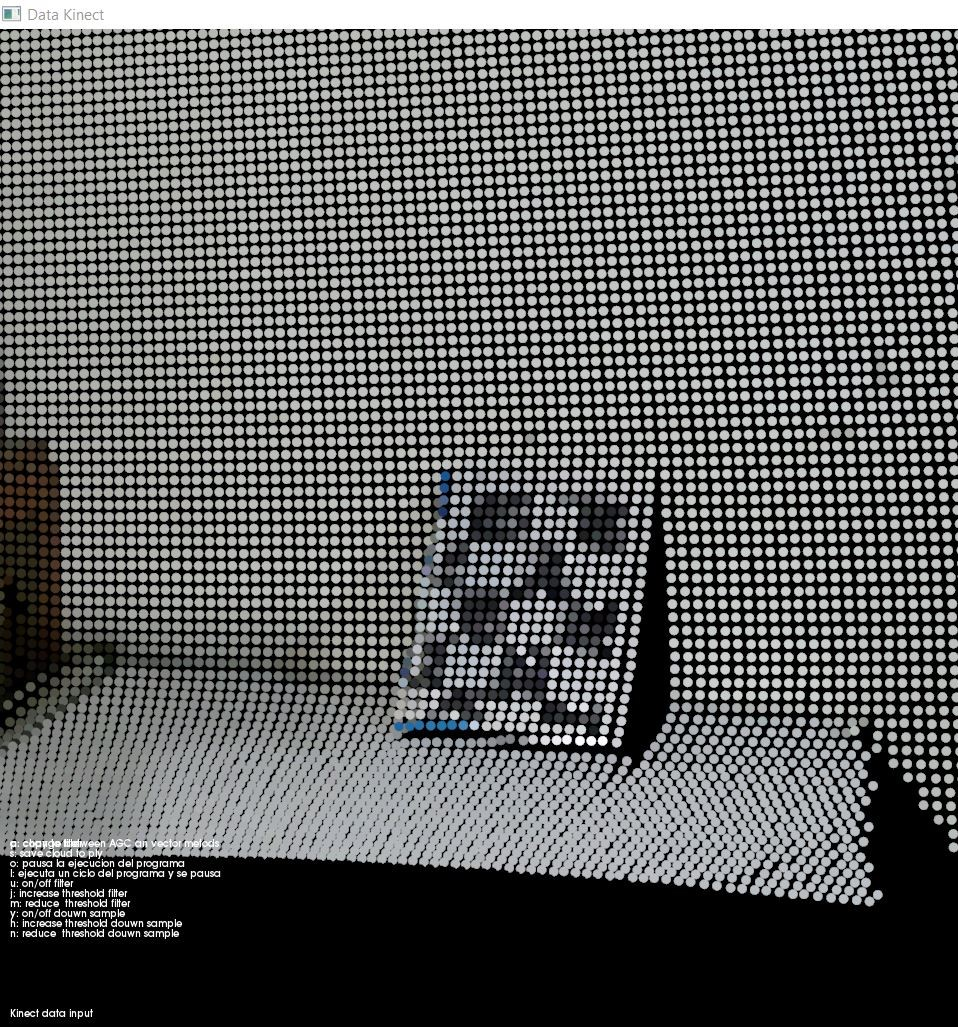
\includegraphics[width=0.45\textwidth]{03Resultados/imagenes/downsampleA.JPG}
		}
		\subfloat[
		\label{fig:coutPointsB}]{%
			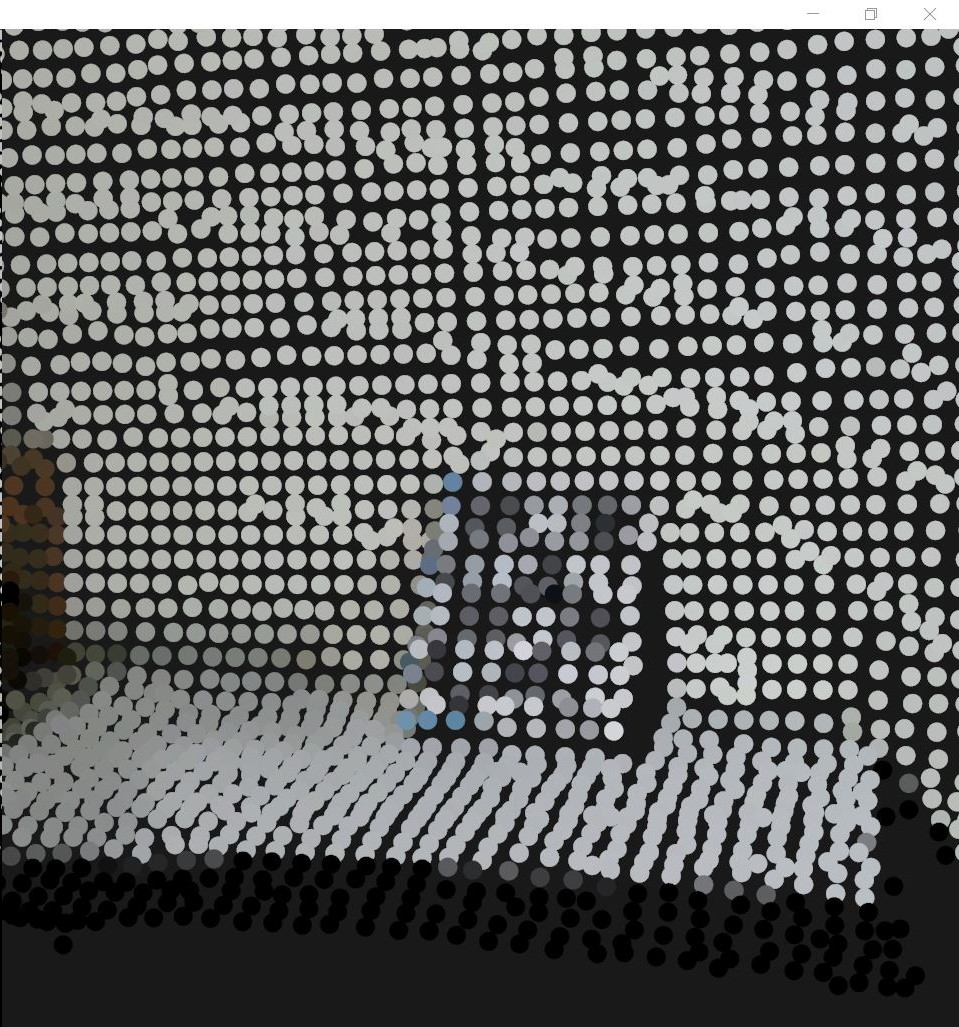
\includegraphics[width=0.45\textwidth]{03Resultados/imagenes/downsampleB.JPG}
		}
		\caption[Prueba para el filtro de densidad de puntos.]{Prueba para el filtro de densidad de puntos, (a) Nube de puntos obtenida del Kinect sobre una cuadrícula de 5cm, (b) Nube de puntos resultante luego del filtro de densidad.}
			\label{fig:coutPoints}
	\end{figure}

%
%	\begin{figure} [!htb]
%		\centering
%		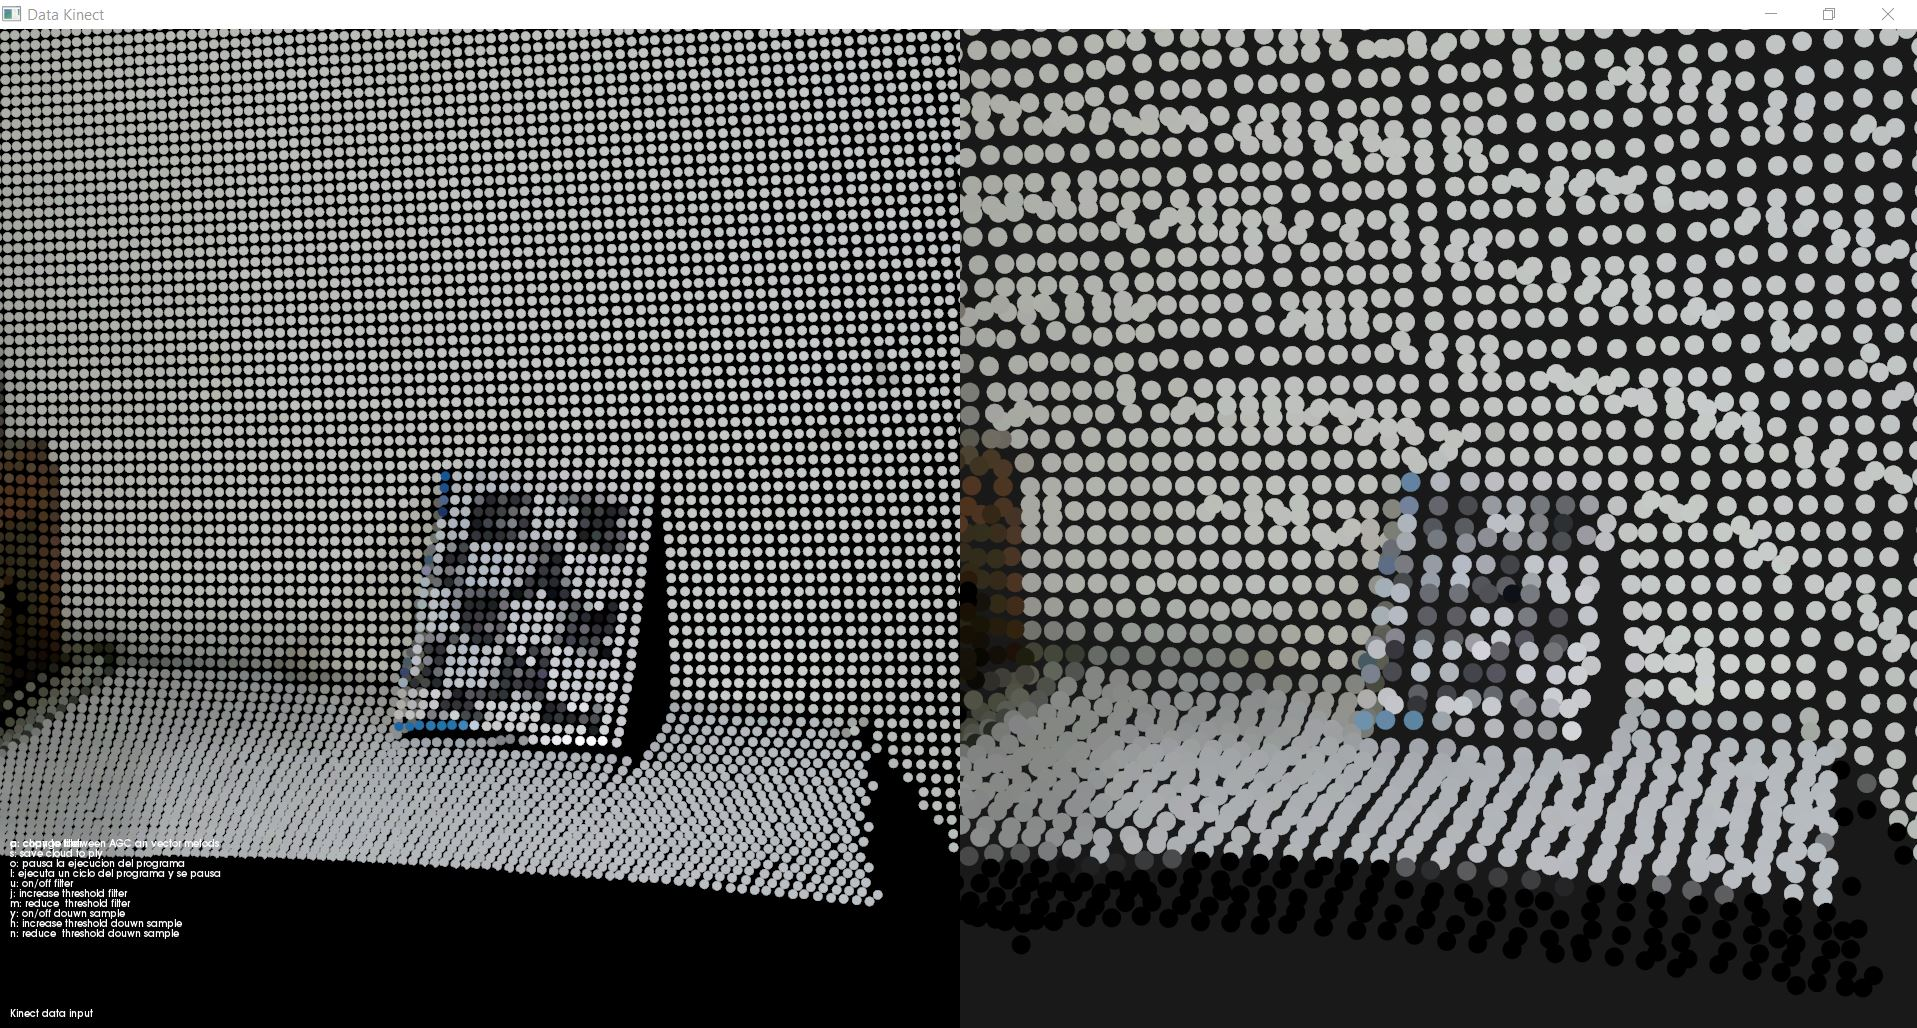
\includegraphics[width=1\textwidth]{03Resultados/imagenes/downsample.JPG}
%		\caption{(izq.)Nube de puntos obtenida del Kinect sobre una cuadrícula de 5cm,(der.)Nube de puntos resultante luego del filtro de densidad.} 
%		\label{fig:coutPoints}
%	\end{figure}
	
	
	\subsection{Por material}
	El Kinect al realizar la detección de profundidad usando ToF depende de la luz infrarroja, si un objeto cuanta con un material que absorbe este tipo de luz el Kinect no será capaz de determinar la nube de puntos. de forma similar ocurre con materiales reflectantes y translucidos.\\
	
\section{Prueba de Segmentación}

	Para el módulo encargado de la segmentación se realizó de una prueba de caja negra para encontrar el espacio de trabajo del sistema. Esta prueba engloba tanto la resta de nubes como el agrupamiento de estos.\\
	\subsection{Escenario}
	Ya que para la segmentación se realiza una resta, es necesario capturar el escenario en el cual trabaja el sistema. Este escenario debe cumplir con una serie de lineamientos:
	\begin{itemize}
		\item No debe estar expuesto a la luz del sol o algún otro emisor de luz infrarroja.
		\item El escenario no debe modificarse mientras el sistema este trabajando.
		\item El escenario no debe contener objetos reflectantes o translucidos.
		\item El escenario debe estar separado del Kinect 0.5m y no estar más alejado de 4.5m.
	\end{itemize}

	\subsection{Objetos}
	\begin{itemize}
		\item El área visible al Kinect debe sobresalir al menos 2.5cm sobre el escenario.
		\item Los objetos deben estar despegados más de 3cm.
	\end{itemize}
	 
\section{Descripción del Caso de Estudio}
	Se planteo el caso de estudio para comparar los dos sistemas propuestos, se busca conocer que método brinda la mejor precisión del sistema para representar correctamente los objetos, y la exactitud al representar cada uno de ellos. Ya que el sistema representa tres tipos de modelos diferentes, se realizo la comparación de los datos para cada uno de los modelos, siendo cada modelo una variable distinta en el caso de estudio, se tienen tres variables, de esta manera se evalúa el sistema dependiendo del modelo esperado, y se obtiene la comparación de los dos métodos para cada modelo propuesto.\\
	
%	El objetivo de esta prueba es el de cuantificar el tiempo, la exactitud y confiabilidad del método elegido así como la modificación realizada con AGC. \\
	
	Antes de continuar hay que aclarar como es que se esta haciendo uso de los conceptos de precisión y exactitud.\\
	
	Para este caso se entiende como precisión a la capacidad del sistema para realizar la clasificación del objeto correctamente, es decir, si el sistema se le presenta el mismo objeto la precisión esta dada por la probabilidad de obtener el mismo tipo de figura en cada ocasión. El sistema es evaluado usando objetos similares a los modelos planteados, cada objeto es evaluado de forma independiente, se le presenta el objeto y se obtiene la decisión tomada por el sistema, este evento es repetido cien veces para obtener la precisión $P$, dada por la división entre la cantidad de veces que el sistema acertó entre el total de intentos del sistema como se muestra en la ecuación \eqref[ec.]{eq:precision}.
	\begin{equation}
	\label{eq:precision}
	P=\frac{\#Aciertos}{\#Intentos}
	\end{equation}
	
	Mientras que exactitud $E$ se entiende como la capacidad del sistema para encontrar el  modelo que mejor representa a la nube de puntos del objeto. Para evaluar la exactitud la prueba se realiza solo cuando el sistema ha seleccionado de manera adecuada el tipo de modelo a usar, si el objeto usado en la evaluación es un balón se obtiene la exactitud solo cuando el sistema decida representarlo como una esfera. La exactitud se obtiene con la ecuación \eqref[ec.]{eq:exactitud} donde $P.Modelo$ es la cantidad de puntos que coinciden con el modelo y $P.Objeto$ es el total de puntos del objeto.
		 
		 \begin{equation}
		 \label{eq:exactitud}
		 E=\frac{P.Modelo}{P.Objeto}
		 \end{equation}
	La obtención de los datos para al evaluación del caso de estudio se realiza de forma similar para cada modelo, por eso solo se explica como se realiza para el caso de la \gls{esfera}, y esto se repite para los modelos del \gls{plano} y el \gls{cilindro}, variando unicamente los objetos usados, para la esfera se uso un balón, para el plano una carpeta de cartón, y para el cilindro una botella de agua. Se eligieron estos objetos ya que presentan una geometría similar a la propuesta, esto representa un caso especial para el sistema ya que con estos objetos se determina que tan capaz es el sistema de excluir a los otros modelos, y se esperaría que el sistema obtenga una capacidad de clasificación por arriba de un $60\%$ al clasificar los objetos, para saber que no son resultados obtenidos de forma aleatoria .\\
	
	Se coloco el sensor Kinect apuntando a una mesa como se muestra en la figura \ref{fig:casoDeESt}. Para el caso de estudio este es el escenario con el cual no se interactúa y que es filtrado usando la resta de nubes de puntos.\\
	
	\begin{figure}[!htb] 
		\centering
		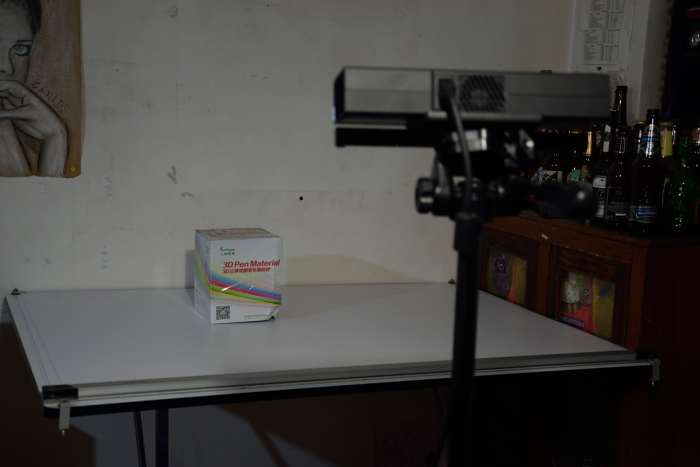
\includegraphics[width=1\textwidth]{03Resultados/imagenes/casoDeEstudio.JPG}
		\caption{Estudio de pruebas} 
		\label{fig:casoDeESt}
	\end{figure}
	
	
	 Se inicia el sistema, y se obtiene la nube de puntos del escenario, luego se coloca el balón sobre la mesa, como se observa en la figura \ref{fig:pruebaEsf}, el sistema realiza el pre-procesamiento y la estimación de los modelos usando RANSAC con los métodos de la biblioteca PCL, se obtienen cien estimaciones del sistema para el balón, y se repite para obtener la estimación usando RANSAC con AGC.\\
	
	
	\begin{figure}[!htb] 
		\centering
		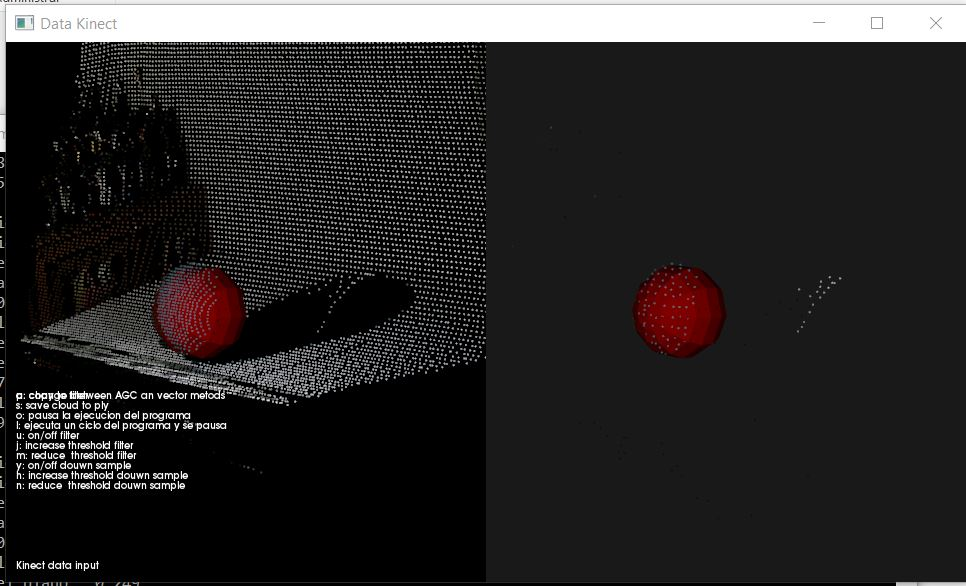
\includegraphics[width=1\textwidth]{03Resultados/imagenes/esfera.JPG}
		\caption{Prueba para la esfera} 
		\label{fig:pruebaEsf}
	\end{figure}
	
	
	Para establecer si los datos obtenidos son diferentes y no eventos aislados se realiza la prueba de suma de rangos de Wilcoxon para datos independientes, para esta prueba se seleccionan los primeros treinta casos en los que el sistema selecciono de manera acertada el tipo de modelo a usar. \\
	
	La prueba de suma de rangos de Wilcoxon se usa para comparar la distribución de grupos de datos, es una prueba no parametrica, es decir que la no se conoce el tipo de distribución de los datos o la distribución de los datos no es normal, siendo la prueba z y la t de Student para datos independientes pruebas equivalentes para datos parameticos, y es para datos independientes ya que los resultados para un método son independientes de los resultados del otro.\cite{bluman2009elementary}.\\
	
	Aplicando la prueba de sumas de rangos de Wilcoxon en el caso de estudio para comparar la exactitud para el modelo de la esfera, primero se establece la hipótesis, ya que se espera una diferencia entre los métodos usados la hipótesis esperada es $H_1:$Los métodos varían en la exactitud obtenida, y la hipótesis nula $H_0:$ No hay diferencia en la exactitud de los métodos.\\
	
	Ya establecida la hipótesis se establece la probabilidad de confianza para la prueba, en este caso se uso una probabilidad de $95\%$ de confianza, lo cual nos da un valor $\alpha=0.05$, y se evalúan las distribuciones tanto por la parte positiva como la negativa se realiza una prueba a dos colas, lo cual usando la distribución normal estándar encontramos que el valor $z$ calculado debe encontrarse en el rango $[-1.96,1.96]$ para afirmar la hipótesis nula, de lo contrario se afirma la hipótesis esperada.\\
	
	Lo siguiente es el calculo y suma de los rangos, para el calculo de los rangos se juntan datos tanto del método AE como los del AGC y se ordenan de mayor a menor y se le asigna un rango iniciando con el dato mas bajo se le asigna el rango uno, al segundo un dos y así hasta el ultimo. si existen datos que tengan el mismo valor, se calcula la media de los rangos y se les asigna la media como rango para todos, por ejemplo, si existen cuatro valores iguales y los rangos para estos datos corresponden a $4,5,6,7$ se calcula la media $(4+5+6+7)/4=5.5$, y este es usado como el rango para los cuatro valores.\\
	
	Ya que los los datos obtenidos son de igual tamaño no habría problema en usar los rangos de AE o de AGC, pero ya que el método AGC es el que estamos comparando contra el AE, se usaran los datos obtenidos usando AGC. Se calcula $R$ que es la suma de los rangos para el método AGC.\\
	
	El calculo del valor $z$ esta dado por la ecuación \eqref[ec.]{eq:z} donde $\mu_R$ y $\sigma_R$ se calculan con las ecuaciones \eqref[ec.]{eq:mu}, \eqref[ec.]{eq:sigma}, respectivamente, donde $n_1$ y $n_2$ es la cantidad de datos usadas en cada método (treinta para ambos casos).
	
	\begin{equation}
	\label{eq:z}
	z=\frac{R-\mu_R}{\sigma_R}
	\end{equation}
	
	\begin{equation}
	\label{eq:mu}
	\mu_R=\frac{n_1(n_1+n_2+1}{2}
	\end{equation}
	
	\begin{equation}
	\label{eq:sigma}
	\sigma_R=\sqrt{\frac{n_1n_2(n_1+n_2+1)}{12}}
	\end{equation}
	
	
	Ya que se usaron treinta casos para AE y otros treinta para AGC $n_1=n_2=30$.
	
	
	 
	\begin{equation}
	\mu_r=915, \sigma_R= 67.6387
	\end{equation}
	 
	 
	 
	 
	 
	 
	 
	 
	 
	 
	 
	 
	 
	 
	 
	
	Ya que el método RANSAC varía los tiempos dependiendo de que tan cerca este de encontrar un modelo que se ajuste a la nube de puntos, se considero realizar una comparación de la media de los tiempos de ejecución.\\
	
	 El proceso que realiza el sistema se dividió en ocho etapas que se describen en la tabla \ref{tab:DefTiempos}. y Se midieron los tiempos a la vez que se obtuvieron los datos para la precisión, dando un conjunto de cien datos para cada modelo y método usado.
	%hacer tabla
	
	\begin{table}[!htb]
		\caption{Descripción de los tiempos del sistema}
		\centering
		\begin{tabular}{ll}
		\hline
		 T1:& La obtención de los datos de sensor Kinect.\\
		 T2:& El filtrado de densidad de puntos.\\
		 T3:& La resta de nubes de puntos.\\
		 T4:& El agrupamiento de los puntos por objeto.\\
		 T5:& Método RANSAC para la esfera.\\
		 T6:& Método RANSAC para el plano.\\
		 T7:& Método RANSAC para el cilindro.\\
		 T8:& Renderizado del resultado.\\
		
		\hline
	\end{tabular}
\label{tab:DefTiempos}
\end{table}
	
	Se realizaron seis casos, tres modelos distintos usando los métodos AE y AGC, Las tablas de los tiempos para cada caso se puede consultar en el apéndice \ref{A:pruebas}.
	


La prueba para el \gls{plano} de realizo colocando un libro (objeto plano) como se muestra en la figura \ref{fig:pruebaPla}.


\begin{figure}[!htb] 
	\centering
	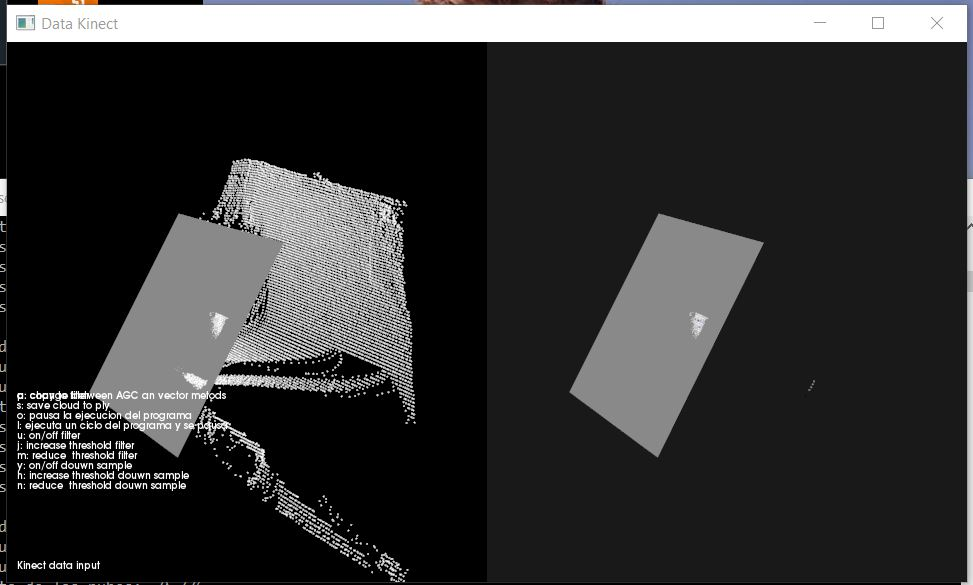
\includegraphics[width=1\textwidth]{03Resultados/imagenes/plano.JPG}
	\caption{Prueba para el plano} 
	\label{fig:pruebaPla}
\end{figure}


Y la prueba para el \gls{cilindro} se realizo colocando un  termo cilíndrico como se muestra en la figura \ref{fig:pruebaCyl}.


\begin{figure}[!htb] 
	\centering
	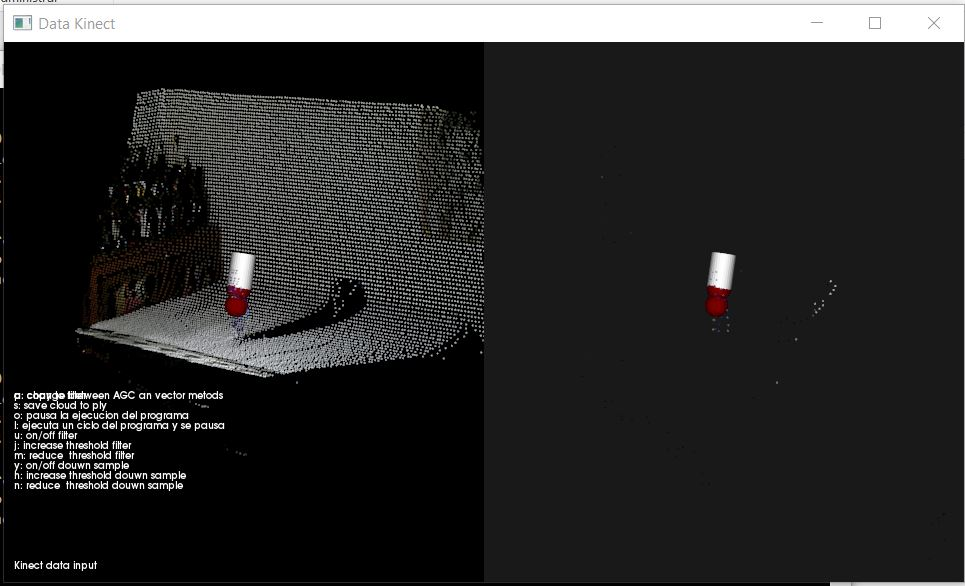
\includegraphics[width=1\textwidth]{03Resultados/imagenes/cilindro.JPG}
	\caption{Prueba para el cilindro} 
	\label{fig:pruebaCyl}
\end{figure}











%recisar la expicacion de las pruebas


%que es la exactitud y la precicion
%como se obtienen


	 
	 
	 
	 
	 
	 
%
%	Uno de los objetivos específicos de este trabajo es el desarrollo de un sistema capaz de obtener datos del sensor Kinect. Esta prueba se diseño para conocer el tiempo requerido por el sensor para realizar el muestreo. El muestreo es independiente al método y en este trabajo se considera una contante.\\
%	
%	El tiempo de muestreo es importante ya que forma parte del ciclo de trabajo y al ser constante el tiempo de respuesta del sistema siempre sera mayor.\\
%	
%	La prueba se lleva acabo sobre el sistema establece la comunicación con el sensor Kinect, crea una nube de puntos con los datos obtenidos, los muestra en pantalla. El tiempo de obtención de datos se mide luego de la conexión con el Kinect hasta antes de que se muestre la nube de puntos en la pantalla.\\
%	
%%	como se muestra en la tabla \ref{tab:planoAGC}.
%%	
%
%\section{Clasificación}
%	Esta prueba se realizo para conocer el tiempo necesario para realizar la clasificación usando RANSAC con AE y que tan precisa y confiable es la clasificación.\\
%	
%	Usando objetos semejantes a las geometrías a clasificar, se colocan uno por vez frente al Kinect para obtener la clasificación del sistema, así como también se calcula que tan representativo es el modelo obtenido comparando el total de puntos en el objeto contra los puntos pertenecientes al modelo.\\
%	
%	
%	
%\subsection{Implementan de AE}
%	La prueba primero se realiza sobe los modelos en AE 
%
%
%\subsection{Implementan de AGC}
%	Para probar el método usando AGC se realiza la misma prueba que en AE para poder coparar los resultados mas adelante.
%	
%\section{Segmentación}
%	Aunque la segmentación se incorporo al sistema desde antes de la clasificación las pruebas de esta no serian relevantes hasta decidir el método de  clasificar a los objetos. ya que la clasificación de un objeto de tarda $t$ tiempo la clasificación se dos seria en $2t$ y así sucesivamente.
	